\documentclass[12pt]{article}
 
\usepackage[margin=1in]{geometry}
\usepackage{amsmath,amsthm,amssymb, mathtools}
\usepackage[T1]{fontenc}
\usepackage{lmodern}
\usepackage{fixltx2e}
\usepackage[shortlabels]{enumitem}
\usepackage{pgfplots}                                                           
\usepackage{pgf}
\usepackage{tikz}                                                               
\usepackage{float}
\usepackage{graphicx}
\graphicspath{ {./} }  
 
\newcommand{\N}{\mathbb{N}}
\newcommand{\R}{\mathbb{R}}
\newcommand{\Z}{\mathbb{Z}}
\newcommand{\Q}{\mathbb{Q}}
\newcommand{\rpm}{\sbox0{$1$}\sbox2{$\scriptstyle\pm$}
  \raise\dimexpr(\ht0-\ht2)/2\relax\box2 }
\newcommand{\norm}[1]{\left\lVert#1\right\rVert}

 
\newenvironment{theorem}[2][Theorem]{\begin{trivlist}
\item[\hskip \labelsep {\bfseries #1}\hskip \labelsep {\bfseries #2.}]}{\end{trivlist}}
\newenvironment{lemma}[2][Lemma]{\begin{trivlist}
\item[\hskip \labelsep {\bfseries #1}\hskip \labelsep {\bfseries #2.}]}{\end{trivlist}}
\newenvironment{exercise}[2][Exercise]{\begin{trivlist}
\item[\hskip \labelsep {\bfseries #1}\hskip \labelsep {\bfseries #2.}]}{\end{trivlist}}
\newenvironment{problem}[2][Problem]{\begin{trivlist}
\item[\hskip \labelsep {\bfseries #1}\hskip \labelsep {\bfseries #2.}]}{\end{trivlist}}
\newenvironment{question}[2][Question]{\begin{trivlist}
\item[\hskip \labelsep {\bfseries #1}\hskip \labelsep {\bfseries #2.}]}{\end{trivlist}}
\newenvironment{corollary}[2][Corollary]{\begin{trivlist}
\item[\hskip \labelsep {\bfseries #1}\hskip \labelsep {\bfseries #2.}]}{\end{trivlist}}
\newcommand{\textfrac}[2]{\dfrac{\text{#1}}{\text{#2}}}

\begin{document}

\title{Numerical Analysis: Homework \#5}

\author{Chris Hayduk}
\date{\today}

\maketitle

\begin{problem}{1}
\end{problem}

\begin{enumerate}
	\item[a)] To minimize the size of the error, we need to minimize the absolute value of,
	\begin{align*}
		\omega(x) = (x - x_0)(x - x_1)(x - x_2)(x - x_3)(x - x_4)(x - x_5)
	\end{align*}
	on $-1 \leq x \leq 1$.\\\\
	We can see that $\omega(x)$ is a monic polynomial of degree 6. Thus, from Theorem 4.5.3, we have,
	\begin{align*}
		\omega(x) = \frac{T_6(x)}{2^5} = \frac{T_6(x)}{32}
	\end{align*}
	Let $n = 6$. Then,
	\begin{align*}
		T_6(x) = 2xT_5(x) - T_4(x)
	\end{align*}
	and,
	\begin{align*}
		T_5(x) = 2xT_4(x) - T_3(x)
	\end{align*}
	From (4.87) and Example 4.5.2, this yields,
	\begin{align*}
		T_5(x) &= 2x(8x^4 - 8x^2 + 1) - (4x^3 - 3x)\\
		&= 16x^5 - 16x^3 + 2x - 4x^3 + 3x\\
		&= 16x^5 - 20x^3 + 5x
	\end{align*}
	And thus we get,
	\begin{align*}
		T_6(x) &= 2x(16x^5 - 20x^3 + 5x) - (8x^4 - 8x^2 + 1)\\
		&= 32x^6 - 40x^4 + 10x^2 - 8x^4 + 8x^2 - 1\\
		&= 32x^6 - 48x^4 + 18x^2 - 1
	\end{align*}
	Thus, we need to minimize,
	\begin{align*}
		\omega(x) = \frac{32x^6 - 48x^4 + 18x^2 - 1}{32}
	\end{align*}
	The node points are the zeros of $\omega(x)$ and from (4.96), they must be the zeros of $T_6(x)$.\\\\
	From definition (4.84) and (4.85), we know that,
	\begin{align*}
		T_6(x) = cos(6\theta), \quad x = cos(\theta)
	\end{align*}
	This expression is zero when,
	\begin{align*}
		&6\theta = \rpm \frac{\pi}{2}, \rpm \frac{3\pi}{2}, \rpm \frac{5\pi}{2}, \rpm \frac{7\pi}{2}, ...\\
		&\theta = \rpm \frac{\pi}{12}, \rpm \frac{3\pi}{12}, \rpm \frac{5\pi}{12}, \rpm{7\pi}{12}, ...\\
		&x = \cos(\frac{\pi}{12}), \cos(\frac{3\pi}{12}), \cos(\frac{5\pi}{8}), \cos(\frac{7\pi}{8}), \cos(\frac{9\pi}{8}), ...
	\end{align*}
	The first six values of $x$ are distinct, but the successive values repeat the first four values. Thus, when we evaluate (4.97), the nodes are approximately,
	\begin{align*}
			\rpm 0.258819, \rpm 0.707107, \rpm 0.965926
	\end{align*}
	Thus, we now have,
	\begin{align*}
			f(x) - P_5(x) &= \frac{(x - x_0)(x - x_1)(x - x_2)(x - x_3)(x - x_4)(x - x_5)}{6!}f^{(6)}(c_x)\\
			&= \frac{x^6 - 2.22045*10^{-16}x^5 - 1.5x^4 + 0.5625x^2 - 1.38778*10^{-17}x - 0.03125}{720}f^{(6)}(c_x)\\
	\end{align*}
	Let's graph the first part of this function,\\\\
	\begin{figure}[H]
	\centering
	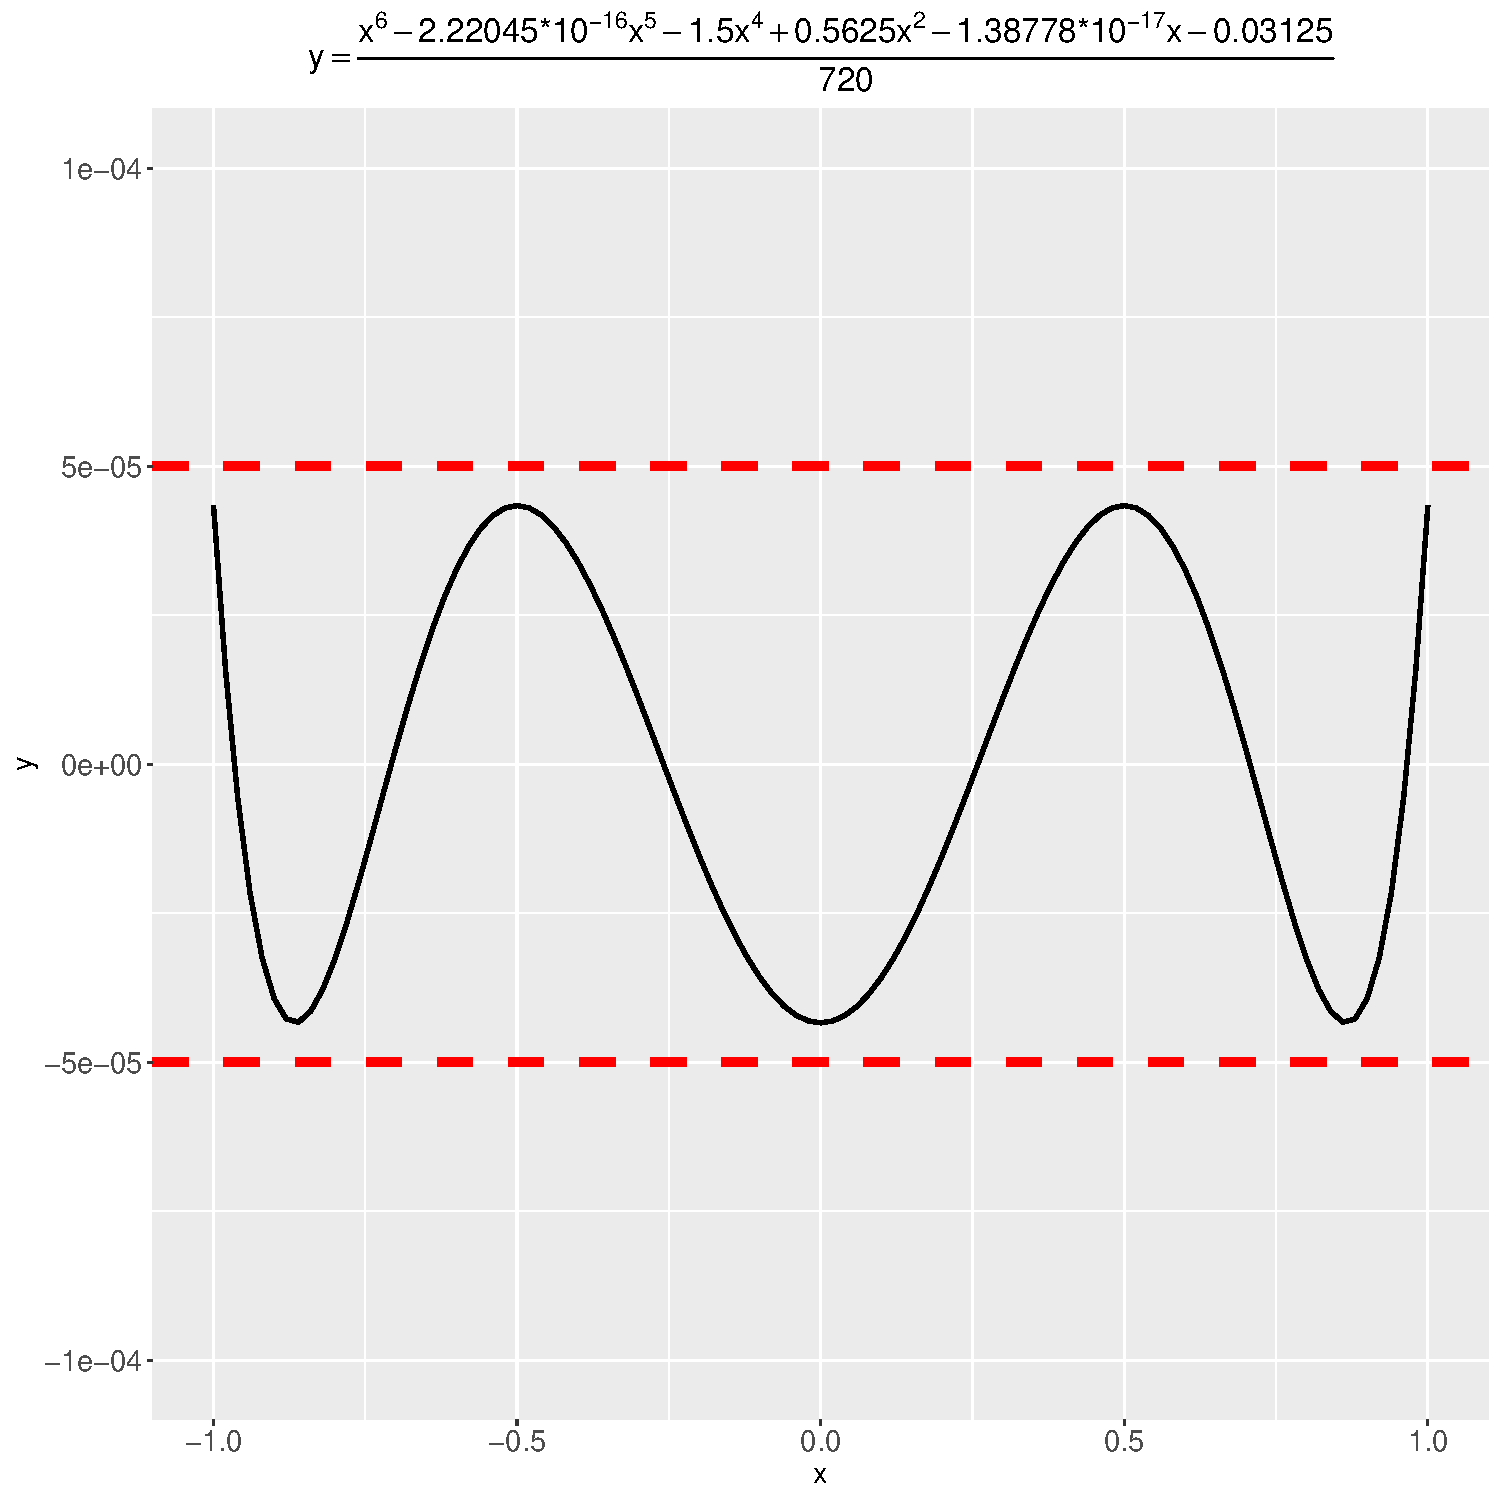
\includegraphics[scale=0.6]{graph}
	\end{figure}
	As can be seen from the graph, 
	\begin{align*}
		\left|\frac{x^6 - 2.22045*10^{-16}x^5 - 1.5x^4 + 0.5625x^2 - 1.38778*10^{-17}x - 0.03125}{720}\right| \leq 5*10^{-5}
	\end{align*}
	when $-1 \leq x \leq 1$.\\
	
	Let's now find a bound for the sixth derivative of $f(x) = e^{2x}$ on $x \in [-1, 1]$.
	\newpage
	\begin{align*}
		&f'(x) = 2e^{2x}\\
		&f''(x) = 2(2e^{2x}) = 4e^{2x}\\
		&f'''(x) = 4(2e^{2x}) = 8e^{2x}\\
		&...\\
		&f^{(6)}(x) = 2^6e^{2x} = 64e^{2x}
	\end{align*}
	It is clear that $e^{2x}$ is an increasing function of $x$. Thus, this equation takes on its maximum value when $c_x = 1$. Plugging into the equation yields,
	\begin{align*}
		f^{(6)}(1) &= 64e^{2} \approx 472.89959 \leq 473
	\end{align*}
	
	Now that we have an upper bound for both terms in the error equation on $x \in [-1, 1]$, we can find an upper bound for the error of $P_5(x)$,
	\begin{align*}
			\left|f(x) - P_5(x)\right| &= \left|\frac{(x - x_0)(x - x_1)(x - x_2)(x - x_3)(x - x_4)(x - x_5)}{6!}f^{(6)}(c_x)\right|\\
			&\leq \left|5*10^{-5}*473\right| = 0.02365\\
	\end{align*}
	Thus, we now have $0.02365$ as an upper bound for the error $\left|f(x) - P_5(x)\right|$ on $x \in [-1, 1]$.
	
	\item[b)] If we use a minimax approximation of $f(x)$, then we have,
	\begin{align*}
			\rho(f) &\leq \frac{[(1 - (-1))/2]^{n+1}}{(n+1)!2^n} \max_{-1 \leq x \leq 1} \left|f^{(n+1)}(x)\right|\\
			&= \frac{1}{(n+1)!2^n} \left|2^{n+1}e^{2}\right|\\
			&= \frac{2e^2}{(n+1)!}
	\end{align*}
	Thus, we need to find $n$ such that,
	\begin{align*}
		\frac{2e^2}{(n+1)!} &\leq 10^{-6}\\
		\implies (n+1)! &\geq \frac{2e^2}{10^{-6}} \approx 14,778,000
	\end{align*}
	From this, we can see that $n = 10$ results in an error less than or equal to $10^{-6}$ on $[-1, 1]$.
\end{enumerate}
\newpage
\begin{problem}{2}
\end{problem}

\begin{enumerate}
	\item[a)] 
	\begin{align*}
		\widetilde{T}_n(x) &= \frac{1}{2^{n-1}}T_n(x)\\
		&= \frac{1}{2^{n-1}}\cos(n\cos^{-1}x)
	\end{align*}
	We know that we need,
	\begin{align*}
		&\left|\cos(m\cos^{-1}x)\right| = 1\\
		\implies &(m\cos^{-1}x) = 0, \quad (m\cos^{-1}x) = \pi\\
		\implies &\cos^{-1}x = 0, \quad \cos^{-1}x = \frac{\pi}{m}\\
		\implies &x = 1, \quad x = \cos\left(\frac{\pi}{m}\right)
	\end{align*}
	Thus, $x = \cos(\frac{\pi}{m})$ for every $m = 1, 2, 3, ..., n$ and $x = 1$ results in, 
	\begin{align*}
		\left|\widetilde{T}_n(x)\right| &= \left|\frac{1}{2^{n-1}}T_n(x)\right|\\
		&= 1
	\end{align*}
	Hence, there are $n + 1$ such points on $[-1, 1]$.
	\item[b)]
	\item[c)] Since both $\widetilde{T}$ and $p(x)$ are both degree $n$ monic polynomials, we know that,
	\begin{align*}
		r(x) &= \widetilde{T} - p(x)\\
		&= (x^n) + \text{lower-degree terms from} \, \widetilde{T} - ((x^n) + \text{lower-degree terms from} \, p(x)\\
		&= \text{lower-degree terms from} \, \widetilde{T} - \text{lower-degree terms from} \, p(x)
	\end{align*}
	Thus, we can see that $r(x)$ has degree $\leq n-1$. Hence, $r$ cannot have $n$ distinct roots and $r(x) = 0$. As a result, $\widetilde{T}(x) = p(x)$.
\end{enumerate}

\begin{problem}{3}
\end{problem}

\begin{enumerate}
	\item[a)] 
	\begin{align*}
		dist(\vec{v}, \vec{v}) &= \norm{\vec{v} - \vec{v}}\\
		&= \norm{\vec{0}} = 0
	\end{align*}
	\item[b)]
	\begin{align*}
		dist(\vec{v}, \vec{w}) &= \norm{\vec{v} - \vec{w}}\\
		&= \norm{(v_1 - w_1, v_2 - w_2, v_3 - w_3, ..., v_n - w_n)}\\
		&= \norm{(-w_1 + v_1, -w_2 + v_2, -w_3 + v_3, ..., -w_n + v_n)}\\
		&= \norm{-1(w_1 - v_1, w_2 - v_2, w_3 - v_3, ..., w_n - v_n)}\\
		&= \norm{-1(\vec{w} - \vec{v})}\\
		&= |-1| \norm{\vec{w} - \vec{v}}\\
		&= \norm{\vec{w} - \vec{v}}
	\end{align*}
	\item[c)]
	\begin{align*}
		dist(\vec{v}, \vec{w}) &= \norm{\vec{v} - \vec{w}}\\
		&= \norm{\vec{v} + (-\vec{w})}\\
		&= \norm{\vec{v} + (-\vec{x} + \vec{x}) + (-\vec{w})}\\
		&= \norm{\vec{v} -\vec{x} + \vec{x} - \vec{w}}\\
		&\leq \norm{\vec{v} -\vec{x}} + \norm{\vec{x} - \vec{w}}\\
		&= dist(\vec{v}, \vec{x}) + dist(\vec{x}, \vec{w})
	\end{align*}
\end{enumerate}

\begin{problem}{4}
\end{problem}


\begin{problem}{5}
\end{problem}

\begin{enumerate}
	\item[a)] 
	\begin{align*}
		\norm{A}_{\infty} &= \max |a_{ij}|\\
		&= 3
	\end{align*}
	\item[b)]
	\begin{align*}
		\norm{A}_{1} &= \sum |a_{ij}|\\
		&= |1| + |2| + |1| + |2| + |2| + |3| + |-1| + |-3| + |0|\\
		&= 15
	\end{align*}
	\item[c)]
	\begin{align*}
		\norm{A}_{2} &= \sqrt{\sum a_{ij}^2}\\
		&= \sqrt{1^2 + 2^2 + 1^2 + 2^2 + 2^2 + 3^2 + (-1)^2 + (-3)^2 + 0^2}\\
		&= \sqrt{33} \approx 5.74456
	\end{align*}
	\item[d)]
	\begin{align*}
		\norm{A}_{h} &= \max_{1 \leq i \leq 3} (\sum_{j=1}^{3} |a_{ij}|)\\
		&= \max [(|1| + |2| + |1|), (|2| + |2| + |3|), (|-1|, |-3|, |0|)]\\
		&= \max [4, 7, 4]\\
		&= 7
	\end{align*}
\end{enumerate}

\end{document}